%% Separately authored additions after exact Relevance and Linear Logic restoration.
% Necessity: the exact inherited chapter does not contain the ternary-incidence
% figure, matched E/R/RM cards and results, IMLL card, full CLL and Lambek
% treatments, or the comparison/consequence apparatus below.
% Definition: this editorial derivative descends from six historical ranges and
% includes current card, theorem, calculus, comparison, and source-role repairs;
% altered ranges are not literal slices.
% Standing: it is editorial reader material, not inherited source or a silent
% proof-status promotion.
% Nonredundancy: the twelve exact wrappers provide both source semantics and the
% IMLL theorem/sketch; these slices retain distinct figures, cards, later systems,
% and apparatus while the historical body and annex remain pinned and unreachable.
% Use: parts/p08.tex inputs this file once after SRC-14069-14094; route, slice,
% label, consumer, and publication tests fail closed on any drift.
\noindent\textit{Reader note.} The following figure, system cards, full CLL and
Lambek treatments, and comparison apparatus are separately attributed
additions to the exact inherited chapter above; they neither replace nor alter
its semantics, calculus, theorem, example, warning, or exercises.

% BEGIN HISTORICAL DERIVATIVE 125-145
\begin{figure}[!htbp]
\centering
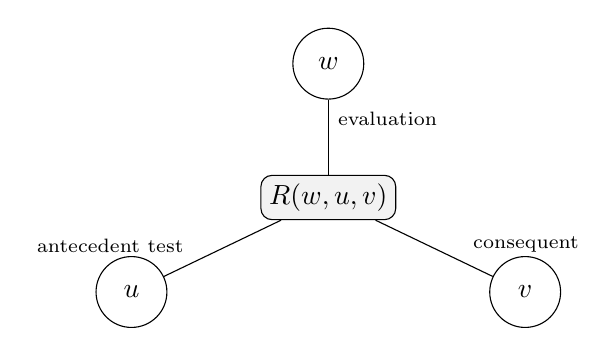
\begin{tikzpicture}[
  world/.style={circle,draw,minimum size=9mm,inner sep=1pt},
  rel/.style={draw,rounded corners,fill=black!5,align=center,
    inner sep=3pt}]
  \node[world] (w) at (0,1.7) {$w$};
  \node[world] (u) at (-2.5,-1.2) {$u$};
  \node[world] (v) at (2.5,-1.2) {$v$};
  \node[rel] (r) at (0,0) {$R(w,u,v)$};
  \draw (w) -- node[right,near start]{\scriptsize evaluation} (r);
  \draw (u) -- node[above left,near start]{\scriptsize antecedent test} (r);
  \draw (v) -- node[above right,near start]{\scriptsize consequent} (r);
\end{tikzpicture}
\caption{One ternary incidence.  The three undirected
incidence lines form one hyperedge recording the ordered tuple \(R(w,u,v)\);
they are not binary accessibility arrows.  The implication clause tests
\(A\) at \(u\) and requires \(B\) at \(v\), with \(w\) as its evaluation
coordinate.}
\label{fig:p08-rm-ternary}
\end{figure}
% END HISTORICAL DERIVATIVE 125-145

% BEGIN HISTORICAL DERIVATIVE 161-341
\begin{hbdefinition}{def:p08-pointed-rm-frame}{Matched relevance frames}
A \emph{pointed Routley--Meyer frame} is
\(\mathfrak F=(K,R,0,{*})\), with nonempty \(K\), distinguished
\(0\in K\), ternary \(R\), and star on \(K\).  Define
\(a\leq b\) iff \(R(0,a,b)\), and set
\[
\begin{aligned}
 R^2(ab)cd &\quad\text{ iff }\quad
   \exists x\,(R(a,b,x)\land R(x,c,d)),\\
 R^2a(bc)d &\quad\text{ iff }\quad
   \exists x\,(R(b,c,x)\land R(a,x,d)),\\
 R^2b(ac)d &\quad\text{ iff }\quad
   \exists x\,(R(a,c,x)\land R(b,x,d)),\\
 R^2abbc &\quad\text{ iff }\quad
   \exists x\,(R(a,b,x)\land R(x,b,c)).
\end{aligned}
\]
These are metalinguistic abbreviations for composite ternary conditions, not
new accessibility relations.

The cited modular presentation uses the base conditions
\begin{align*}
 \mathrm{B1}:&\ a\leq a,\\
 \mathrm{B2}:&\ a\leq b\land b\leq c\text{ implies }a\leq c,\\
 \mathrm{B3}:&\ a'\leq a\land R(a,b,c)\text{ implies }R(a',b,c),\\
 \mathrm{B4}:&\ a^{**}=a,\\
 \mathrm{B5}:&\ a\leq b\text{ implies }b^*\leq a^*.
\end{align*}
The labels are metalinguistic names for the five displayed frame conditions,
not object-language schemas.  Its \(\mathbf E\)-frames satisfy
B1--B5 and, universally,
\[
\begin{gathered}
 \mathrm{E3}:\ R^2(ab)cd\text{ implies }R^2a(bc)d,\qquad
 \mathrm{E4}:\ R^2(ab)cd\text{ implies }R^2b(ac)d,\\
 \mathrm{E5}:\ R(a,b,c)\text{ implies }R^2abbc,\qquad
 \mathrm{E6}:\ R(a,0,a).
\end{gathered}
\]
Its \(\mathbf R\)-frames are those \(\mathbf E\)-frames also
satisfying \(\mathrm{R7}: R(a,b,c)\text{ implies }R(b,a,c)\).  Its
\(\mathbf{RM}\)-frames additionally satisfy
\(\mathrm{M}: 0\leq a\) or \(0\leq a^*\), for every \(a\).  A valuation is
hereditary along \(\leq\), and the satisfaction clauses are those of
Section~\ref{sec:relevance-linear-02}; formula validity is truth at the
distinguished point \(0\).  These are semantic frame classes matched to the
three exact sheets, not the broad class above
\cite{RoutleyMeyer1973,DunnRestall2002}.  A different direct R-frame package
uses period two together with an inversion condition; it is not silently
combined with this modular B1--B5/E3--E6/R7/M presentation.
\index{pointed Routley--Meyer frame}
\end{hbdefinition}

\begin{systementry}{entry:p08-relevance-r}{Relevant implication \(\mathbf R\)}
  \index{relevance logic!R}
  \entryaliases{\(\mathbf R\), the Anderson--Belnap system of relevant
    implication.}
  \entrylanguage{Constant-free formulas over propositional variables, with
    primitive \(\neg,\land,\lor,\to\).}
  \entrysemantics{The matched pointed \(\mathbf R\)-frames of
    Definition~\ref{def:p08-pointed-rm-frame}, with hereditary valuations and
    validity at \(0\).}
  \entrycalculus{sheet:relevance-r}
  \entryadequacy{cited=DunnRestall2002}{Formula theoremhood is sound and
    complete for the matched pointed \(\mathbf R\)-models.  This is not an
    arbitrary-premise local-consequence theorem for the broad frames.}
  \entrydecidability{cited=Urquhart1984}{Full propositional \(\mathbf R\)
    theoremhood is undecidable.  This status does not classify the distinct
    pure implicational fragment; its positive result is stated separately
    below.}
  \entrycharacteristic{It has variable sharing for theorem implications,
    admits Ackermann's theoremhood metarule \(\gamma\), and rejects the
    irrelevant weakening example; these claims retain their separate
    hypotheses below.}
  \entrytranslations{The correspondence cells in
    Table~\ref{tab:p08-relevance-systems} use the composite-relation
    abbreviations of Definition~\ref{def:p08-pointed-rm-frame}.}
  \entrysources{AndersonBelnap1975,RoutleyMeyer1973,DunnRestall2002,Urquhart1984}
\end{systementry}

\begin{hbtheorem}{thm:p08-relevance-adequacy}{cited=DunnRestall2002}{Relevance theoremhood adequacy}
For \(X\in\{\mathbf E,\mathbf R,\mathbf{RM}\}\), let the calculus and
pointed frame class be exactly those fixed by the corresponding registry sheet
and Definition~\ref{def:p08-pointed-rm-frame}.  Then
\[
 \derives_X A\quad\text{ iff }\quad\entails_X A
\]
for formula theoremhood.  The statement does not identify theoremhood with an
arbitrary-premise relevant consequence relation and does not apply to the
broad frames of Section~\ref{sec:relevance-linear-02}.
\end{hbtheorem}

\begin{hbtheorem}{thm:p08-relevance-variable-sharing}{cited=AndersonBelnap1975}{Variable sharing for \(\mathbf E\) and \(\mathbf R\)}
Let \(A\) and \(B\) be constant-free formulas.  If
\(\derives_{\mathbf E} A\to B\) or
\(\derives_{\mathbf R} A\to B\), then \(A\) and \(B\) have a propositional
variable in common.  This is a theoremhood property of implications, not an
arbitrary-premise consequence theorem and not a sufficient definition of
relevance.
\end{hbtheorem}

\begin{hbtheorem}{thm:p08-rm-variable-sharing}{cited=DunnRestall2002}{R-mingle and variable sharing}
Full \(\mathbf{RM}\) does not have the variable-sharing property above;
\(\neg(p\to p)\to(q\to q)\) is a standard counterexample.  The safe weaker
statement is: if \(A\to B\) is an \(\mathbf{RM}\)-theorem, then either
\(A\) and \(B\) share a variable, or both \(\neg A\) and \(B\) are
\(\mathbf{RM}\)-theorems.
\end{hbtheorem}

\begin{hbdefinition}{def:p08-ackermann-gamma}{Ackermann's gamma metarule}
Ackermann's \emph{gamma metarule} is the theoremhood-preservation condition
that theoremhood of \(A\) and of \(\neg A\lor B\) entails theoremhood of
\(B\).  Its standing is an admissible metarule, not a primitive object-language
schema or a rule from open assumptions.  The name is necessary to distinguish
this condition from modus ponens, whose conditional premise is \(A\to B\),
and from unrestricted disjunctive syllogism.  It is used in the next theorem
and Table~\ref{tab:p08-relevance-systems}.
\index{Ackermann gamma}
\end{hbdefinition}

\begin{hbtheorem}{thm:p08-gamma-admissibility}{cited=MeyerDunn1969}{Gamma admissibility for \(\mathbf E\) and \(\mathbf R\)}
For \(X\in\{\mathbf E,\mathbf R\}\), if
\(\derives_X A\) and \(\derives_X\neg A\lor B\), then
\(\derives_X B\).  Gamma is not added to either registry sheet: the theorem
says that the metarule preserves theoremhood.  No theory-uniform
\(\mathbf{RM}\) generalization is asserted here.
\end{hbtheorem}

\begin{hbtheorem}{thm:p08-relevance-undecidable}{cited=Urquhart1984}{Undecidability of \(\mathbf E\) and \(\mathbf R\)}
The theoremhood problems for full propositional \(\mathbf E\) and
\(\mathbf R\) are undecidable.  This theorem concerns the full languages; it
does not concern only their pure implicational fragments and supplies no
decision classification for \(\mathbf{RM}\).
\end{hbtheorem}

\begin{hbtheorem}{thm:p08-relevance-implicational-decidable}{cited=DunnRestall2002}{Decidable pure implicational fragments}
The theoremhood problems for the pure implicational fragments
\(\mathbf E_{\to}\) and \(\mathbf R_{\to}\) are decidable.  Their restricted
input languages make this result consistent with
Theorem~\ref{thm:p08-relevance-undecidable}.
\end{hbtheorem}

\begin{hbtheorem}{thm:p08-rm-decidable}{cited=Avron2016}{Decision boundary for \(\mathbf{RM}\)}
Full propositional \(\mathbf{RM}\) is decidable and has the finite-model
property.  This classification is distinct from Urquhart's theorem for
\(\mathbf E\) and \(\mathbf R\) and is also recorded in the standard survey
\cite{DunnRestall2002}.
\end{hbtheorem}

\begin{table}[!htbp]
\centering
\begingroup\scriptsize
\setlength{\tabcolsep}{3pt}
\begin{tabular}{@{}p{.08\textwidth}p{.15\textwidth}p{.15\textwidth}
  p{.23\textwidth}p{.13\textwidth}p{.13\textwidth}@{}}
\toprule
System & Exact sheet & Distinguishing surface & Matched pointed-frame addition
& Variable sharing & Gamma status \\
\midrule
\(\mathbf E\) & \texttt{relevance-e} & Fixed-menu \(\mathbf E\) schemas and
MP/adjunction & Composite associativity/permutation, contraction, point, and
star clauses in Definition~\ref{def:p08-pointed-rm-frame} & yes, for
constant-free theorem implications; Theorem~\ref{thm:p08-relevance-variable-sharing}
& admissible for theoremhood; Theorem~\ref{thm:p08-gamma-admissibility} \\
\(\mathbf R\) & \texttt{relevance-r} & \(\mathbf E\) plus Demodaliser & \(\mathbf E\) conditions plus
  \(R(a,b,c)\text{ implies }R(b,a,c)\) & yes, with the same scope & admissible for
theoremhood \\
\(\mathbf{RM}\) & \texttt{relevance-rm} & \(\mathbf R\) plus Mingle & \(\mathbf R\) conditions plus
\(0\leq a\) or \(0\leq a^*\) & no; weak replacement in
Theorem~\ref{thm:p08-rm-variable-sharing} & no theory-uniform claim; the
package does not promote gamma to a primitive rule \\
\bottomrule
\end{tabular}
\endgroup
\caption{Named relevance systems, controlled by
\cite{AndersonBelnap1975,MeyerDunn1969,RoutleyMeyer1973,DunnRestall2002}.
Formula schemas remain exclusively on the named sheets.  ``Gamma'' means the
theoremhood metarule in Definition~\ref{def:p08-ackermann-gamma}, not ordinary
modus ponens.}
\label{tab:p08-relevance-systems}
\end{table}
% END HISTORICAL DERIVATIVE 161-341

% BEGIN HISTORICAL DERIVATIVE 398-423
\begin{systementry}{entry:p08-imll}{Intuitionistic multiplicative linear logic}
  \index{intuitionistic multiplicative linear logic}
  \entryaliases{\(\mathsf{IMLL}\); the tensor--unit--linear-implication
    core only.}
  \entrylanguage{Atoms, \(\mathbf 1\), \(A\otimes B\), and
    \(A\multimap B\); no additives, exponentials, or primitive linear
    negation.}
  \entrysemantics{Commutative residuated partially ordered monoids, with
    finite-multiset antecedents interpreted by their tensor product.}
  \entrycalculus{sheet:imll}
  \entryadequacy{proved=annex:p08-imll-complete}{The calculus is sound and
    complete for the displayed algebras, and cut is admissible in its
    cut-free fragment, by \cref{thm:p08-imll-complete}. The inherited
    sketch is retained separately at
    \cref{thm:p08-imll-historical-sketch}.}
  \entrydecidability{proved=annex:p08-imll-np-complete}{Derivability for this
    exact calculus is NP-complete by \cref{thm:p08-imll-np-complete}.
    The proof gives polynomial cut-free certificates and an explicit
    unary 3-PARTITION reduction using only two atoms, \(\otimes\), and
    \(\multimap\).}
  \entrycharacteristic{Exchange is built into multiset contexts; unrestricted
    weakening and contraction are absent.}
  \entrytranslations{The source-bounded bang extension below has a distinct
    sheet and does not inherit this card's adequacy status.}
  \entryalgebra{Commutative residuated partially ordered monoids.}
  \entrysources{Girard1987,GalatosJipsenKowalskiOno2007,Lincoln1995,GareyJohnson1979}
\end{systementry}
\section{The multiplicative core: adequacy and complexity}
\label{sec:p08-imll-complete}

The result concerns exactly \hyperref[sheet:imll]{the registered IMLL calculus}: one succedent, finite
multiset antecedents, and the connectives \(\mathbf1,\otimes,\multimap\).
It does not cover the subsequent exponential extension.
The algebraic interpretation and empty-context convention are those of
\cref{sec:relevance-linear-03,def:p08-imll-empty-tensor}.

\begin{hbtheorem}{thm:p08-imll-historical-sketch}{sketched=annex:p8.imll.source}{Source claim}
The inherited result at
\hyperref[thm:p08-source-imll-adequacy]{Soundness, completeness, and cut elimination}
announces adequacy for commutative residuated partially ordered monoids
and admissibility of cut. Its adjacent argument is a sketch.
The following theorem supplies the complete argument for the same
multiplicative calculus, separately from the historical sketch.
\end{hbtheorem}

\begin{hbtheorem}{thm:p08-imll-complete}{proved=annex:p08-imll-complete}{Soundness completeness and cut elimination for IMLL}
For a finite multiset \(\Gamma\) and a formula \(A\) of
\hyperref[sheet:imll]{the registered IMLL calculus}, the following are equivalent:
\begin{enumerate}
 \item \(\Gamma\Rightarrow A\) has a derivation in that calculus.
 \item \(\Gamma\Rightarrow A\) has a cut-free derivation.
 \item In every commutative residuated partially ordered monoid and
       every valuation, the product of the values in \(\Gamma\)
       is below the value of \(A\).
\end{enumerate}
The product of an empty antecedent is the monoid unit.
No weakening, contraction, distributive lattice structure, or
exponential operation is assumed.
\end{hbtheorem}

\begin{hbmethod}{def:p08-imll-cut-procedure}{Eliminating a cut}
First eliminate cuts in the immediate subderivations. For a remaining
cut with cut-free premises, mark the particular occurrence of its
cut formula in the right premise. If an identity ends either premise,
remove the cut directly. Otherwise commute the cut above a last rule
that does not introduce its marked formula. If both last rules
introduce that formula, replace a tensor cut by two cuts on its factors,
an implication cut by cuts on its domain and codomain, and a unit cut
by the right premise before unit insertion. The proof establishes all
these cases. A lexicographic induction on formula size and the sum of
premise heights proves termination. The procedure does not copy or
discard resources; equal formula occurrences remain separately marked.
\end{hbmethod}

The canonical algebra in the proof is a countermodel method as well:
if a sequent is not derivable, the quotient of formulas by mutual
derivability, with atoms interpreted by their own classes, falsifies it.
This is an existence construction, not a claim of an efficient finite
countermodel algorithm. The inherited algebraic and proof-theoretic
setting is discussed in \cite{Girard1987,GalatosJipsenKowalskiOno2007}.

\begin{hbtheorem}{thm:p08-imll-proof-bound}{proved=annex:p08-imll-proof-bound}{Finite proof search and polynomial certificates}
Let \(N\) be the total number of atom, connective and unit occurrences
in an input sequent of \hyperref[sheet:imll]{the registered IMLL calculus}. Every cut-free proof of it
has at most \(N\) nodes. Exhaustive backward search over the registered
cut-free rules terminates and decides derivability. With an effective
finite-string encoding of atoms and formulas, a successful proof has
polynomial encoded size and is checkable in polynomial time.
Consequently derivability belongs to \(\mathsf{NP}\).
This proves membership, not the separate NP-hardness assertion.
\end{hbtheorem}

\subsection{The lower complexity bound}

\begin{hbdefinition}{def:p08-imll-partition-encoding}{The partition encoding}
For a formula \(A\) and a positive integer \(n\), let \(A^{\otimes n}\)
denote a fixed parenthesization of \(n\) copies of \(A\), not an additional
connective.  A unary 3-PARTITION instance consists of positive integers
\(m,B,a_1,\ldots,a_{3m}\), with
\[
 \sum_{i=1}^{3m}a_i=mB,\qquad B/4<a_i<B/2,
\]
written in unary.  Its question is whether the indices can be partitioned
into \(m\) triples, each having sum \(B\).  For distinct atoms \(p,q\), put
\[
 F_i=p^{\otimes a_i}\multimap q,\qquad
 D=p^{\otimes B}\multimap q^{\otimes3}.
\]
The encoded sequent is
\[
 F_1,\ldots,F_{3m}\Rightarrow D^{\otimes m}.
\]
Repeated numerical values still give separate antecedent occurrences.
\end{hbdefinition}

\begin{hbtheorem}{thm:p08-imll-partition}{proved=annex:p08-imll-partition}{Correctness of the encoding}
The sequent in \cref{def:p08-imll-partition-encoding} is derivable in
\hyperref[sheet:imll]{the registered IMLL calculus} if and only if its
3-PARTITION instance has a solution.  The translation has length
\(O(mB+m)\) and is polynomial-time for unary input.
\end{hbtheorem}

\begin{hbcorollary}{thm:p08-imll-np-complete}{proved=annex:p08-imll-np-complete}{NP-completeness}
Derivability in the registered IMLL calculus is NP-complete under
polynomial-time many-one reductions.  Hardness already holds for the
two-atom, unit-free sequents of \cref{def:p08-imll-partition-encoding}.
\end{hbcorollary}

The hardness premise is the strong NP-completeness of 3-PARTITION,
equivalently the NP-completeness of its unary version; its source is
\textcite[Theorem~4.4]{GareyJohnson1979}.  The encoding and its converse
are proved here.  Unary encoding matters: expanding a binary integer
into that many tensor factors would not in general be polynomial.


% END HISTORICAL DERIVATIVE 398-423

% BEGIN HISTORICAL DERIVATIVE 453-715

\section{Full one-sided classical linear logic}
\label{sec:p08-cll}

The full classical system is independent new depth material.  It does not use
the IMLL annex item as evidence.

\begin{hbdefinition}{def:p08-cll-language}{CLL formulas and linear negation}
The cited one-sided CLL presentation has paired atoms
\(p,p^\perp\), multiplicative units \(\mathbf 1,\bot\), additive units
\(\top,0\), and are closed under
\(\otimes,\bindnasrepma,\mathbin{\&},\oplus,!,?\).  Formula-level
\emph{linear negation} is the involution fixed on atoms and by
\[
\begin{gathered}
 (A\otimes B)^\perp=A^\perp\bindnasrepma B^\perp,
 \qquad
 (A\bindnasrepma B)^\perp=A^\perp\otimes B^\perp,\\
 \mathbf 1^\perp=\bot,\quad \bot^\perp=\mathbf 1,\qquad
 (A\mathbin{\&}B)^\perp=A^\perp\oplus B^\perp,\\
 (A\oplus B)^\perp=A^\perp\mathbin{\&}B^\perp,
 \qquad \top^\perp=0,\quad 0^\perp=\top,\\
 (!A)^\perp=?A^\perp,\qquad(?A)^\perp=!A^\perp.
\end{gathered}
\]
This name is necessary to distinguish an operation on formulas from Routley
star and from phase orthogonality on sets.  Its standing is a syntactic De
Morgan operation, not ordinary object-language falsum; it differs from
primitive negation in the relevance language and is used by the one-sided
sheet, connective table, and phase interpretation.  Linear implication is the
defined connective \(A\multimap B\defeq A^\perp\bindnasrepma B\).
\index{linear negation}
\index{classical linear logic}
\end{hbdefinition}

\begin{hbdefinition}{def:p08-focusing-polarity}{Andreoli focusing polarity}
In Andreoli's one-sided focusing convention used for the displayed CLL
presentation, a formula constructor is
\emph{positive} when its introduction is assigned to a synchronous focused
phase, and \emph{negative} when its introduction is assigned to an
asynchronous phase whose available introduction is invertible.  The positive
nullary connective \(0\) has no introduction rule, so the first clause does
not assert that every positive constructor supplies an applicable rule.  Each
atom receives a declared polarity, and its formal linear negation receives the
opposite polarity.  This is a metalinguistic classification used to schedule
focused proof search, not an object-language connective or a semantic truth
value.  The name is necessary to distinguish the synchronous/asynchronous
proof-search discipline from De Morgan duality and from positive or negative
truth; those classifications do not determine one another.  Table
\ref{tab:p08-linear-connectives} uses the distinction to record the source
constructor classes \cite{Andreoli1992}.
\index{focusing polarity}
\end{hbdefinition}

\begin{table}[!htbp]
\centering
\begingroup\small
\setlength{\tabcolsep}{3pt}
\begin{tabular}{@{}p{.18\textwidth}p{.22\textwidth}p{.19\textwidth}
  p{.14\textwidth}p{.16\textwidth}@{}}
\toprule
Symbol & CLL role & De Morgan dual & Focusing polarity & In IMLL card? \\
\midrule
\(\otimes\) & multiplicative conjunction & \(\bindnasrepma\) & positive & yes \\
\(\bindnasrepma\) & multiplicative disjunction (par) & \(\otimes\) & negative & no \\
\(\mathbf 1\) & tensor unit & \(\bot\) & positive & yes \\
\(\bot\) & par unit & \(\mathbf 1\) & negative & no \\
\(\mathbin{\&}\) & additive conjunction (with) & \(\oplus\) & negative & no \\
\(\oplus\) & additive disjunction (plus) & \(\mathbin{\&}\) & positive & no \\
\(\top\) & with unit & \(0\) & negative & no \\
\(0\) & plus unit & \(\top\) & positive & no \\
\(!\) & bang exponential & \(?\) & positive & no \\
\(?\) & quest exponential & \(!\) & negative & no \\
\(A^\perp\) & formula linear negation & \((A^\perp)^\perp=A\) & reverses
the declared polarity & no primitive counterpart \\
\bottomrule
\end{tabular}
\endgroup
\caption{Linear-logic connective registry.  The polarity
column follows Andreoli's focusing convention \cite{Andreoli1992}; it is not
a truth-value classification.  Each atom receives a declared polarity and its
formal negation receives the opposite polarity.}
\label{tab:p08-linear-connectives}
\end{table}

\begin{hbdefinition}{def:p08-phase-space}{Full-CLL phase semantics}
A \emph{phase space}, in Girard's notation, is a pair \((M,\perp)\), where
\(M\) is a commutative monoid written multiplicatively, with unit \(1\), and
\(\perp\subseteq M\) is the \emph{pole}.  For \(X,Y\subseteq M\), define the
phase-subset residual and phase orthogonal by
\[
 X\multimap Y
 =\{m\in M:\forall x\in X\
      (mx\in Y)\},
 \qquad
 X^{\perp}
 =X\multimap\perp.
\]
A \emph{fact} is a subset \(X\subseteq M\) with
\(X=X^{\perp\perp}\).  Here the source uses the same glyph
\({}^{\perp}\) for formula negation and subset orthogonality; the operand type
makes the two roles exact.  These names are needed
to distinguish the semantic model, its designated orthogonality test, and its
closed semantic values from formula-level linear negation.  Here \(\perp\) is
locally typed as a subset of \(M\), not as the formula-level par unit.  Their standing is
semantic: the residual is a typed operation on phase subsets, the pole is a
subset of phases, and a fact is a closed subset, not a formula or a proof
object.  The phase residual differs from formula-level \(\multimap\) by its
subset operands, and is used to define phase orthogonality.  The distinctions
are used in every interpretation clause and in
Theorem~\ref{thm:p08-phase-adequacy}.

Interpret atoms as facts.  Following Girard, write \(A^*\) for the fact
interpreting formula \(A\), and use the connective glyphs themselves for the
corresponding operations on facts:
\[
\begin{aligned}
 X\otimes Y&=\{xy:
                     x\in X, y\in Y\}^{\perp\perp},
 &X\bindnasrepma Y&=(X^\perp\otimes Y^\perp)^\perp,\\
 (\mathbf 1)^*&=\{1\}^{\perp\perp},
 &\bot^*&=\{1\}^{\perp},\\
 X\mathbin{\&}Y&=X\cap Y,
 &X\oplus Y&=(X\cup Y)^{\perp\perp},\\
 \top^*&=M,
 &0^*&=\varnothing^{\perp\perp}.
\end{aligned}
\]
For the exponentials define the idempotent phase set
\[
 I=\{m\in\{1\}^{\perp\perp}:mm=m\},
\]
and set
\[
 !X=(X\cap I)^{\perp\perp},
 \qquad
 ?X=(X^\perp\cap I)^\perp.
\]
The set \(I\) is required for the cited phase interpretation; omitting
it would define only an exponential-free phase semantics.  A formula \(A\) is
\emph{phase-valid} iff \(1\in A^*\) in every such interpretation.  This
validity differs from membership in one phase
model and is the notion used in the next theorem \cite{Girard1995}.
\index{phase semantics}
\index{fact!linear logic}
\end{hbdefinition}

\begin{systementry}{entry:p08-cll}{One-sided classical linear logic}
  \index{classical linear logic!one-sided calculus}
  \entryaliases{\(\mathsf{CLL}\), with full multiplicatives, additives,
    units, and exponentials.}
  \entrylanguage{The formulas and involutive linear negation of
    Definition~\ref{def:p08-cll-language}; one-sided judgments have finite
    multiset contexts.}
  \entrysemantics{The phase models of
    Definition~\ref{def:p08-phase-space}, including the idempotent-phase
    clauses for bang and quest.}
  \entrycalculus{sheet:cll-one-sided}
  \entryadequacy{cited=Girard1995}{Cut is eliminable and formula theoremhood
    is sound and complete for the displayed phase semantics.}
  \entrydecidability{cited=LincolnMitchellScedrovShankar1992}{Full
    propositional CLL is undecidable.  Its exponential-free
    multiplicative--additive fragment is PSPACE-complete, and its
    multiplicative fragment is NP-complete.}
  \entrycharacteristic{No unrestricted weakening or contraction is present;
    the quest-prefixed structural rules are explicit on the sheet.}
  \entrytranslations{\(A\multimap B\defeq
    A^\perp\bindnasrepma B\); the IMLL card is a different, single-succedent
    intuitionistic calculus.}
  \entryalgebra{Phase spaces and their biorthogonally closed facts.}
  \entrysources{Girard1987,Girard1995,Andreoli1992,LincolnMitchellScedrovShankar1992}
\end{systementry}

\begin{hbtheorem}{thm:p08-cll-cut-elimination}{cited=Girard1995}{CLL cut elimination}
Every sequent derivable on \hyperref[sheet:cll-one-sided]{the registered
one-sided CLL sheet} has a cut-free derivation.  Equivalently, its displayed
cut rule is admissible in the cut-free fragment.  This cited theorem covers
the exact multiplicative, additive, unit, and exponential surface of that
sheet; it is not inherited from the IMLL sketch.
\end{hbtheorem}

\begin{hbtheorem}{thm:p08-phase-adequacy}{cited=Girard1995}{Phase soundness and completeness}
For every formula \(A\) in the displayed full propositional CLL language,
\[
 \derives_{\mathsf{CLL}}A
 \quad\text{ iff }\quad
 1\in A^*
 \text{ in every displayed phase interpretation}.
\]
The theorem is formula theoremhood.  The exponential clauses and idempotent
phase set in Definition~\ref{def:p08-phase-space} are part of its hypotheses;
an MALL-only interpretation may not be advertised as this full result.
\end{hbtheorem}

\begin{hbtheorem}{thm:p08-linear-decision-boundaries}{cited=LincolnMitchellScedrovShankar1992}{Linear-logic decision boundaries}
Full propositional linear logic with exponentials is undecidable.  Its
fragment with multiplicatives and additives but no exponentials is
PSPACE-complete, while the multiplicative fragment is NP-complete.  These are
three distinct input languages and do not transfer a decision result to the
source's unnamed four-rule bang extension.
\end{hbtheorem}

\section{The associative Lambek calculus}
\label{sec:p08-lambek}

\begin{hbdefinition}{def:p08-lambek-semantics}{Lambek L and its algebra}
Lambek's \emph{associative calculus \(\mathsf L\)} has formulas
generated from atoms by product \(A\mathbin{\cdot}B\), left division
\(A\backslash B\), and right division \(B/A\).  Antecedents are finite
nonempty ordered sequences; the calculus has no exchange, weakening,
contraction, empty antecedent, or multiplicative unit.  This exact name is
necessary to distinguish \(\mathsf L\) from \(\mathsf L^*\), which permits
empty antecedents, and from \(\mathsf L_1\), which adds a unit.  Its standing
is the proof system on \hyperref[sheet:lambek-l]{the Lambek sheet}, and the
distinction is used in its card and complexity statement.

A \emph{residuated semigroup} is a partially ordered semigroup
\((U,\mathbin{\cdot},\leq)\) with residuals satisfying
\[
 a\mathbin{\cdot}b\leq c
 \quad\text{ iff }\quad
 b\leq a\backslash c
 \quad\text{ iff }\quad
 a\leq c/b.
\]
Its standing is algebraic semantics, not syntax; unlike the IMLL algebra it
need not be commutative or have a unit.  A sequent
\(A_1,\ldots,A_n\Rightarrow B\) is valid iff
\(v(A_1)\mathbin{\cdot}\cdots\mathbin{\cdot}v(A_n)\leq v(B)\) under every
valuation in every such semigroup \cite{Lambek1958,Buszkowski2010}.
\index{Lambek calculus}
\index{residuated semigroup}
\end{hbdefinition}

\begin{systementry}{entry:p08-lambek-l}{Associative Lambek calculus L}
  \index{Lambek calculus!system entry}
  \entryaliases{\(\mathsf L\); unit-free, nonempty-antecedent associative
    Lambek calculus.}
  \entrylanguage{Atoms, product, left division, and right division.}
  \entrysemantics{Residuated semigroups, interpreting the ordered antecedent
    by its left-to-right semigroup product.}
  \entrycalculus{sheet:lambek-l}
  \entryadequacy{cited=Buszkowski2010}{The calculus is sound and complete for
    the displayed residuated-semigroup semantics, and cut is admissible.}
  \entrydecidability{cited=Pentus2006}{Derivability for \(\mathsf L\) is
    NP-complete.  The same cited paper also treats \(\mathsf L^*\), but that is
    not the card's calculus.}
  \entrycharacteristic{Ordered nonempty antecedents make exchange, weakening,
    contraction, and the empty-context unit unavailable.}
  \entrytranslations{Its two residuals coincide only under an additional
    commutativity assumption, which is absent here.}
  \entryalgebra{Partially ordered residuated semigroups without a required
    unit.}
  \entrysources{Lambek1958,Buszkowski2010,Pentus2006}
\end{systementry}

\begin{hbtheorem}{thm:p08-lambek-adequacy}{cited=Buszkowski2010}{Lambek adequacy and cut elimination}
For the exact unit-free, nonempty-antecedent calculus
\hyperref[sheet:lambek-l]{\(\mathsf L\)}, a sequent is derivable iff it is
valid in every residuated semigroup.  Every derivable sequent also has a
cut-free derivation.  Neither assertion silently changes the calculus to
\(\mathsf L^*\) or \(\mathsf L_1\).
\end{hbtheorem}
% END HISTORICAL DERIVATIVE 453-715

% BEGIN HISTORICAL DERIVATIVE 716-866

\section{Comparison by context profile}

\begin{hbdefinition}{def:p08-affine-family-boundary}{The selected commutative affine calculus}
An \emph{affine} calculus admits unrestricted weakening but not unrestricted
contraction.  The selected presentation here is the commutative affine
intuitionistic linear calculus on
\hyperref[sheet:affine-ill]{\texttt{sheet:affine-ill}}: formulas and
exactly-single-succedent sequents are those of IMLL, antecedents are finite
multisets so exchange is built in, every IMLL rule is retained, and the
registered Weakening rule takes \(\Gamma\Rightarrow B\) to
\(\Gamma,A\Rightarrow B\) for arbitrary \(A\), while contraction remains
absent.

The qualifier ``selected'' is necessary because affine systems can have
different languages and context policies.  It names this exact calculus, not
the entire affine family, and differs from IMLL by the displayed weakening
rule.  The distinction is used in both comparison tables and the structural
map below.  The sheet contains Cut as a rule; no independent affine adequacy or
cut-elimination theorem is asserted here \cite{Lincoln1995}.
\index{affine linear logic}
\end{hbdefinition}

\begin{table}[!htbp]
\centering
\begingroup\scriptsize
\setlength{\tabcolsep}{3pt}
\begin{tabular}{@{}p{.15\textwidth}p{.19\textwidth}p{.12\textwidth}
  p{.13\textwidth}p{.13\textwidth}p{.20\textwidth}@{}}
\toprule
Named system or boundary & Context representation & Exchange & Unrestricted
weakening & Unrestricted contraction & Exact sheet or boundary \\
\midrule
\(\mathbf E\) & Hilbert theorem sequences, not contexted sequents & not a
structural-rule cell & not a structural-rule cell & not a structural-rule cell
& \hyperref[sheet:relevance-e]{\texttt{relevance-e}} \\
\(\mathbf R\) & Hilbert theorem sequences, not contexted sequents & not a
structural-rule cell & not a structural-rule cell & not a structural-rule cell
& \hyperref[sheet:relevance-r]{\texttt{relevance-r}} \\
\(\mathbf{RM}\) & Hilbert theorem sequences, not contexted sequents & not a
structural-rule cell & not a structural-rule cell & not a structural-rule cell
& \hyperref[sheet:relevance-rm]{\texttt{relevance-rm}} \\
\(\mathsf{IMLL}\) & finite multiset antecedent; one succedent & built in &
absent & absent & \hyperref[sheet:imll]{\texttt{imll}} \\
Source bang extension & finite multiset antecedent; one succedent & built in &
bang-prefixed formulas only & bang-prefixed formulas only &
\hyperref[sheet:ill-exponential-extension]{\texttt{ill-exponential-extension}};
no inherited metatheorem \\
One-sided \(\mathsf{CLL}\) & finite multiset, one-sided & built in &
absent; quest-prefixed exception & absent; quest-prefixed exception &
\hyperref[sheet:cll-one-sided]{\texttt{cll-one-sided}} \\
Commutative affine ILL & finite multiset antecedent; one succedent & built in &
present & absent & \hyperref[sheet:affine-ill]{\texttt{affine-ill}};
no adequacy theorem claimed \\
Associative Lambek \(\mathsf L\) & finite nonempty ordered antecedent; one
succedent & absent & absent & absent &
\hyperref[sheet:lambek-l]{\texttt{lambek-l}} \\
\bottomrule
\end{tabular}
\endgroup
\caption{Substructural family map by exact context profile.
The three relevance rows point separately to their exact Hilbert systems;
assigning them one generic sequent profile would fabricate a calculus.
Exponential weakening and contraction are not unrestricted structural rules.}
\label{tab:p08-substructural-family}
\end{table}

\begin{figure}[!htbp]
\centering
\begin{tikzpicture}[
  profile/.style={draw,rounded corners,align=center,inner sep=5pt,
    text width=3.7cm},
  note/.style={draw,dashed,rounded corners,align=center,inner sep=5pt,
    text width=3.7cm},
  >=Latex]
  \node[profile] (comm) {finite multisets\\exchange built in\\no
    unrestricted weakening or contraction\\\(\mathsf{IMLL}\),
    \(\mathsf{CLL}\)};
  \node[profile,right=3.2cm of comm] (aff) {commutative affine ILL\\finite
    multisets; one succedent\\unrestricted weakening present\\contraction
    absent\\\texttt{affine-ill}};
  \node[profile,below=2.0cm of comm] (lambek) {nonempty ordered
    sequences\\remove exchange\\associative Lambek \(\mathsf L\)};
  \node[note,below=2.0cm of aff] (rel) {\(\mathbf E,\mathbf R,\mathbf{RM}\)\\
    exact Hilbert sheets\\system-specific; no structural-deletion arrow};
  \draw[dashed,->] (comm) -- node[above,align=center]{family-level
    contrast:\\add weakening}
    (aff);
  \draw[->] (comm) -- node[left,align=right]{retain order;\\remove exchange}
    (lambek);
\end{tikzpicture}
\caption{Structural-policy map.  Arrows record only a
change in context policy; they are not theorem-set inclusions, translations,
or claims that one logic is obtained from another merely by deleting an LK
rule.  Formula languages and proof-theoretic standings remain those of the
named sheets.}
\label{fig:p08-substructural-family}
\end{figure}

\section{Consequence properties and scope boundary}
\label{sec:p08-substructural-consequence}

\begin{hbdefinition}{def:p08-context-consequence-properties}{Context-sensitive consequence properties}
For a relation between contexts and conclusions, \emph{identity} means that a
formula follows from its singleton context; \emph{context extension} means
that inserting additional occurrences wherever the declared representation
permits preserves derivability; and \emph{cut composition} means that a
derivation of \(A\) may replace a displayed occurrence of \(A\) in another
derivation.  These are metalinguistic properties of a contexted relation.  They
are needed because Tarskian monotonicity for set-valued semantic consequence
forgets order and multiplicity, whereas the calculi below do not.  Thus context
extension is not renamed ``monotonicity'' in the table.  The distinction is
used in the comparison with nonmonotonic retraction below.
\index{monotonicity!context extension}
\index{cut!composition}
\end{hbdefinition}

\begin{table}[!htbp]
\centering
\begingroup\scriptsize
\setlength{\tabcolsep}{3pt}
\begin{tabular}{@{}p{.19\textwidth}p{.20\textwidth}p{.13\textwidth}
  p{.19\textwidth}p{.20\textwidth}@{}}
\toprule
Relation or boundary & Representation & Identity & Context extension & Cut /
transitivity standing \\
\midrule
Set-valued semantic consequence & sets of premises & yes & yes, Tarskian
monotonicity & yes, Tarskian transitivity \\
\(\mathsf{IMLL}\) derivability & finite multisets; one succedent & displayed
on \texttt{imll} & no unrestricted extension & cut displayed; elimination
sketched by \hyperref[entry:p08-imll]{the IMLL card} \\
\(\mathsf{CLL}\) derivability & finite one-sided multisets & displayed on the
\hyperref[sheet:cll-one-sided]{CLL sheet} & no unrestricted extension; quest
exception only &
cut displayed and cited eliminable in
Theorem~\ref{thm:p08-cll-cut-elimination} \\
Commutative affine ILL derivability & finite multisets; one succedent &
displayed on \hyperref[sheet:affine-ill]{\texttt{affine-ill}} &
yes, by unrestricted weakening & Cut displayed; no elimination or adequacy
theorem asserted here \\
Lambek \(\mathsf L\) derivability & finite nonempty ordered sequences &
displayed on \texttt{lambek-l} & no arbitrary insertion or permutation & cut
displayed and cited eliminable in Theorem~\ref{thm:p08-lambek-adequacy} \\
\(\mathbf E,\mathbf R,\mathbf{RM}\) theoremhood & no premise context in the
exact Hilbert sheets & not a context cell & not a context cell & gamma is a
theoremhood metarule, not structural cut \\
\bottomrule
\end{tabular}
\endgroup
\caption{Context-sensitive consequence properties.  Set monotonicity and
occurrence-sensitive context extension are deliberately separate.}
\label{tab:p08-consequence-properties}
\end{table}

Read the structural profiles in Table~\ref{tab:p08-consequence-properties}
together with the distinct
information-retraction objects in
Table~\ref{tab:p08-nonmonotonic-properties}. The comparison does not identify
substructural failure of a rule with nonmonotonic defeat by added information.

% END HISTORICAL DERIVATIVE 716-866

% BEGIN HISTORICAL DERIVATIVE 874-894
The following boundary deliberately does not claim a local correctness
criterion, sequentialization theorem, or net-based cut-elimination proof
beyond the cited source.

\begin{proofboundary}{def:p08-linear-pointer-boundary}{Coherence spaces, proof nets, and excluded developments}
Girard's coherence-space semantics and proof nets are entry points in the
original linear-logic development \cite{Girard1987}.  The recorded
\hyperref[def:p07-proof-nets-goi-boundary]{Part-7 proof-net and geometry-of-interaction
boundary} governs the scope: no proof-net correctness criterion,
sequentialization theorem, net-based cut elimination, or
geometry-of-interaction execution model is developed.  Quantum logic,
adaptive logics, and formal argumentation are also outside this chapter's
technical scope.  For the orthomodular-lattice program of quantum logic see
\textcite{BirkhoffVonNeumann1936}; for the dynamic marking strategy of adaptive
logics see \textcite{Batens2007}; and for abstract argumentation frameworks and
their extension semantics see \textcite{Dung1995}.  These are source-specific
navigation pointers, not imported definitions or theorem claims.
\index{coherence space}
\index{proof net}
\index{geometry of interaction}
\end{proofboundary}
% END HISTORICAL DERIVATIVE 874-894

The finite abstract-argumentation definitions, extension semantics and
complete proofs are supplied separately in
Chapter~\ref{sec:p18-finite-argumentation}.  That treatment preserves the
distinction between extension membership and truth of an argument's premises.
